%%%%%%%%%%%%%%%%%%%%%%%%%%%%%%%%%%%%%%%%%%%%%%%%%%
\chapter{Setup and frameworks}
\label{chap:setup-and-frameworks}

Following the overview of existing gesture recognition techniques in the previous chapter (chapter \ref{chap:gesture-recognition}), this chapter focuses on the hardware and software requirements necessary for implementing a gesture recognition architecture. These requirements will lead to a choice of hardware components and of an ensemble of software libraries to be used in this project. Since there are many software libraries capable of performing the individual tasks of tracking or classification, but not all of them are suited for a real-time-capable integrated architecture, the choice of camera, environment constraints and libraries is greatly influenced by the main requirement of the real-time, or quasi-real-time component of ergonomic gestures.

%%%-%-%-%-%-%-%-%-%-%-%-%%-%-%-%-%-%-%-%-%-%-%-%%%
\section{Hardware}
\label{sec:hardware}

The main task of the hardware is to see a user's hand and fingers positions and movements while this user is sitting in front of the interface. While there are approaches based on accelerometer and gyroscopic sensors 
\cite{dataglove}, this project will focus on a vision-based setup and will therefore use a camera. The interface can be anything from an LCD display to a beamer, as long it is in front of the user and not obstructing the field of view of the camera. In order for a camera to \textit{see} the fingers, several important requirements have to be met for the camera:

\begin{itemize}
\item Resolution: \\ The camera frame must contain enough information about the fingers in order to localize and distinguish them from each other. As ad-hoc tests have shown, resolutions of 320$\times$240 pixels may work, depending of the user's action space and the distance between the camera and the user, but often overstep the threshold of being distinguishable or simply the threshold of detection of the fingers.

\item Frame rate: \\ Even if the recognition of a gesture can operate at a much lower sampling rate while still having enough consecutive samples to identify a gesture reliably (in the range of 5 to 20 frames per second), the articulated and sudden or rapid movements of the hand result in blurred fingers in a single frame taken at up to 30 frames per second \cite{blurry}. Therefore, the camera should acquire the images at a speed where rapid movements can be captured without motion blur (even if each second or third frame will be skipped in the video processing loop).

\item Color and image fidelity: \\ Movements of hands and fingers should not result in distorted images often seen in conventional web-cams. In order to prevent difficulties in the tracking algorithms, the 
camera should have low color shifts and a low noise ratio;
\end{itemize}

Given a camera that meets these requirements and providing a solid basis for the video processing steps, this project further constrains the goal regarding the tracked object: in order to meet the requirement of being able to localize the finger positions in a given image, the user is wearing a glove with marked finger extremeties.

%------------------------------------------------%
\subsection{Camera}
\label{sub:camera}

While most of the conventional USB Web-cameras do not meet the camera requirements established above, the following three cameras, often used in computer vision systems, do.
\begin{itemize}
\item Point Grey FireFly MV (752$\times$480 at 60 FPS) \cite{pointgrey}
\item Unibrain Fire-i (501 Model: 640$\times$480 at 86 FPS) \cite{unibrain}
\item Sony PS3 Eye (640$\times$480 at 75 FPS) \cite{ps3eye}
\end{itemize}

While each of these cameras could be used in this project, the choice fell on the Sony PS3 Eye camera (see figure \ref{fig:ps3-eye}). Its main advantage is its cost, subsidized by Sony for the use with Playstation games, which is under CHF 70.- in most electronics stores.

\begin{figure}[H]
\center
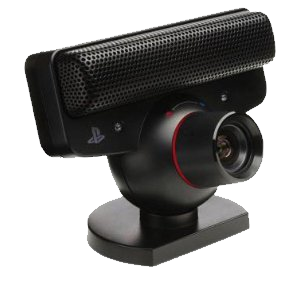
\includegraphics[width=0.3\textwidth]{images/ps3eye} 
\caption{Sony PS3 Eye camera}
\label{fig:ps3-eye}
\end{figure}

While Sony does not provide a driver, a member of the Natural User Interface group \cite{nuigroup} provided a Windows driver that supports frame rates up 75 FPS in VGA (640$\times$480) resolution and up to 120 FPS in QVGA (320$\times$240) resolution \cite{codelab}. The driver is also capable of grabbing frames from multiple cameras in OpenCV under Windows, which could be a requirement for stereoscopy, whereas under other Operating Systems, only one camera was recognized in OpenCV.
 
%------------------------------------------------%
\subsection{Glove}
\label{sub:glove}

The use of a glove facilitates the tracking of the fingers: for the scope of this project, tracking color-based markers on the fingertips presented a acceptable shortcut to obtain the finger positions. \\
The glove was initially designed to put it on and off quickly, without having the disadvantage of placing all the color markers each time on the hand. The design also went through several versions optimizing the placement and color of the markers for better tracking results (see figure \ref{fig:glove}).
The main improvement was obtained by placing the markers on the fingertips in a way that did not cover the whole circumference of the finger, which provided the ability to distinguish the fingers for the tracking phase.

\begin{figure}[H]
   \centering
   \subfloat[1$^{\text{st}}$ version]{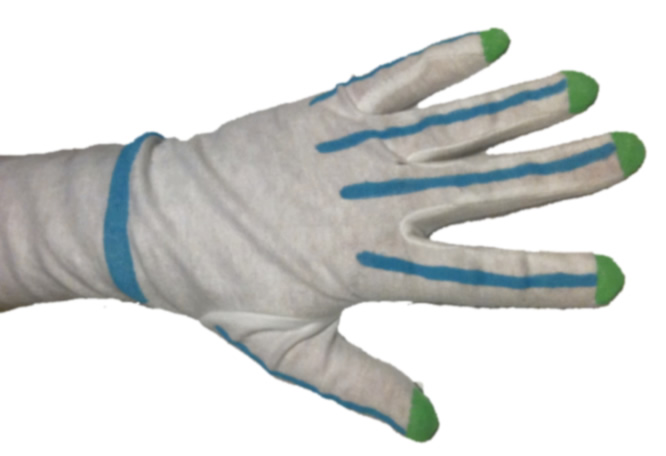
\includegraphics[width=0.25\textwidth]{images/glovev1}}
      \hspace{0.05\textwidth}
   \subfloat[2$^{\text{nd}}$ version]{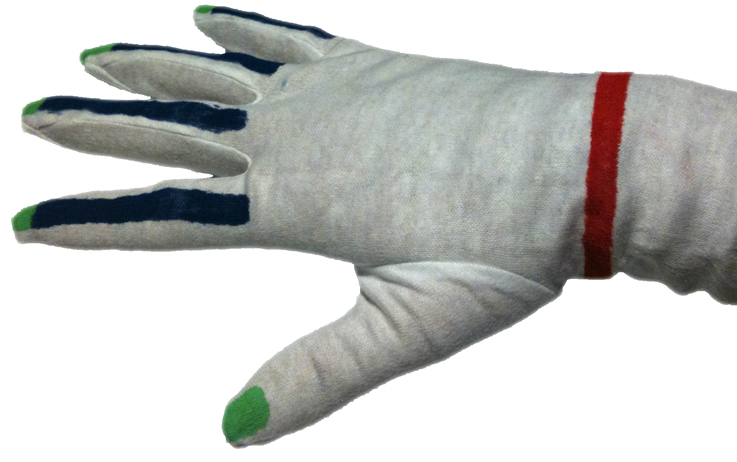
\includegraphics[width=0.25\textwidth]{images/glovev2}}
   	\hspace{0.05\textwidth}
   \subfloat[3$^{\text{rd}}$ version]{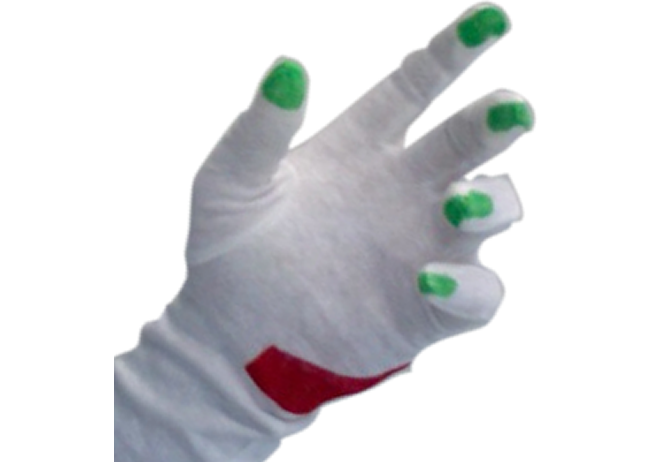
\includegraphics[width=0.25\textwidth]{images/glovev3}}
   \caption{Color-marked textile glove}
   \label{fig:glove}
\end{figure}

%------------------------------------------------%
\subsection{Environmental constraints}
\label{sub:environmental-constraints}

Initially, the following setup had been proposed:
\begin{itemize}
	\item the user is sitting in front of the interface,
	\item while sitting and resting the elbows on the table,
	\item and the camera being placed at a distance where the gestural action space is contained in the field of view of the camera (see figure \ref{fig:setup}).
\end{itemize}

\begin{figure}[H]
\center
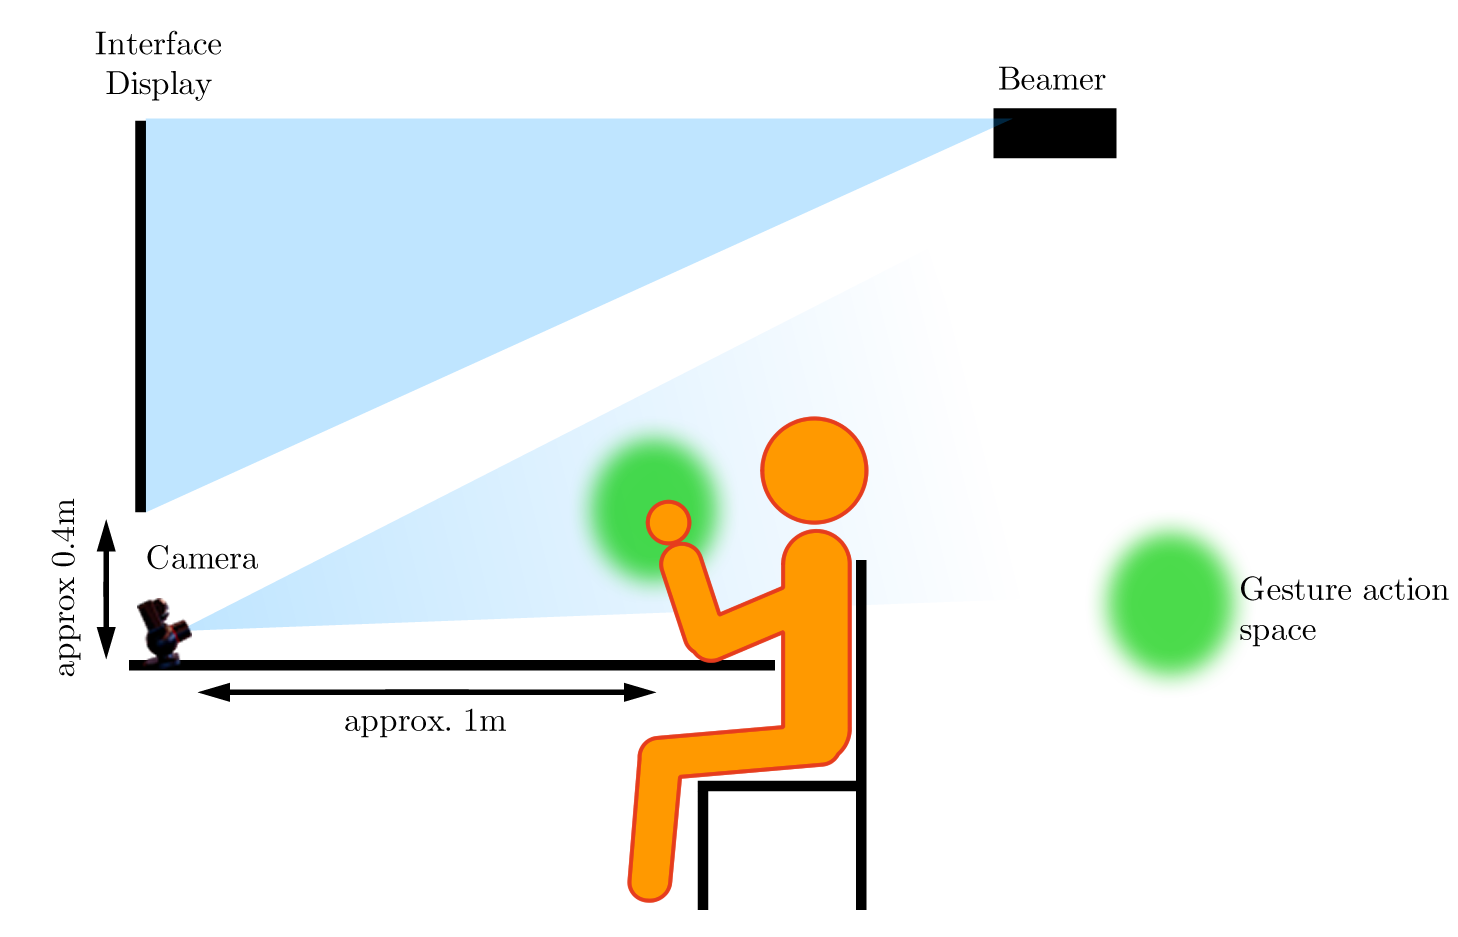
\includegraphics[width=0.9\textwidth]{images/setup} 
\caption{Setup of the interface}
\label{fig:setup}
\end{figure}

While this project aims at recognising hand postures and gestures without too much restricting the setup, some constraints have to be further imposed in order to reliably obtain good tracking and classification results. 

Even if the tracker algorithm operates in a color space that is less dependent of the luminance of the color like HSL or Lab color space, there are some limits due to the gain of the camera: in a very dim lit environment the noise is too much amplified by the gain and the colors are more indistinguishable. Equally, with very bright spots or in direct sunlight, the pixels of the color markers lose their color information, turning to a color value close to white.

The glove's design was optimized for frontal control gestures. The placement of the wrist marker imposes a further environmental constraint: the camera has to be placed lower than the display, allowing it to film in a slightly rising direction and ensuring to capture the wrist markers whenever executing a gesture. But of course color markers on the glove also means that neither the user nor the background can contain these colors.

%%%-%-%-%-%-%-%-%-%-%-%-%%-%-%-%-%-%-%-%-%-%-%-%%%
\section{Software}
\label{sec:software}

The main requirement of the software is to allow real-time tracking and classification. To this regard, the tracking and classification algorithms should be written in C/C++. Of course, other languages might be viable for real-time image processing algorithms, capable of managing threads and offering helping mechanisms like a garbage collector. But initial library tests have shown, especially for image processing algorithms, that with a slightly heightened awareness for memory management, thread management and algorithm execution times, better performances could be achieved more easily with C/C++.

%------------------------------------------------%
\subsection{Overview}
\label{sub:overview}

A library or set of libraries is needed, where the following tasks are covered:

\begin{itemize}
\item fast image processing algorithms
\item ability to train a classifier
\item easily design a performant GUI for rapid application development
\item take advantage of a multicore hardware architecture
\end{itemize}

Due to the chosen hardware (see section \ref{sub:camera}) for which the device driver operates best in the Windows operating system, the choice of the development environment falls to the Visual Studio 2008 IDE. 

%------------------------------------------------%
\subsection{Libraries and frameworks}
\label{sub:libraries-and-frameworks}

\subsubsection{OpenCV}
OpenCV \cite{opencv} is a library containing a large set of algorithms covering computer vision and machine learning tasks. It is a cross-platform library initially developed by Intel and now maintained under active development by Willow Garage \cite{opencv-web}. Its goal was to advance computer vision research and provide a basic infrastructure for computer vision. This library was chosen for its focus on real-time image processing.
The current version is 2.2, however this project used the version 2.0, because at the time of the first integration of the OpenCV algorithms, the tracking was optimized for multithreading using OpenMP instructions. OpenCV abandoned its built-in OpenMP optimizations in favour of TBB (Thread Building Blocks).

\subsubsection{dlibc++}
The dlib library \cite{dlib} was chosen for its well documented usage of Support Vector Machines (SVM). It provides a C++ API for a multitude of binary classifiers and regression tools: Relevance Vector Machines (RVM), kernel recursive least squares (KRLS), kernel ridge regression (KRR) and several implementations of Support Vector Machines.

\subsubsection{QT}
QT \cite{qt} was favored over Windows forms (.NET or MFC) because of the extension possibilities like the integration of OpenGL within QT widgets. The use of OpenGL to display enhanced video frames greatly improves the performance in combination with an OpenGL capable graphics hardware. Furthermore it is an multi-platform and open-source GUI framework.

\subsubsection{libconfig}
Initially the tracker program featured Boost object serialization for saving the states and parameters of the image processing steps. But due to consistency problems a simpler solution was needed. libconfig is a library for reading and writing structured configuration files, with type-awareness, groups, lists, arrays, strings and numbers.

